\documentclass{article}

\usepackage{arxiv}

\usepackage[utf8]{inputenc} % allow utf-8 input
\usepackage[T1]{fontenc}    % use 8-bit T1 fonts
\usepackage{lmodern}        % https://github.com/rstudio/rticles/issues/343
\usepackage{hyperref}       % hyperlinks
\usepackage{url}            % simple URL typesetting
\usepackage{booktabs}       % professional-quality tables
\usepackage{amsfonts}       % blackboard math symbols
\usepackage{nicefrac}       % compact symbols for 1/2, etc.
\usepackage{microtype}      % microtypography
\usepackage{lipsum}
\usepackage{graphicx}

\title{Quantifying effect sizes in implicit learning tasks; the role of
some stuff}

\author{
    Kelly G. Garner
    \thanks{Corresponding author}
   \\
    School of Psychology \\
    University of Birmingham \\
  Edgbaston, UK, B13 2TT \\
  \texttt{\href{mailto:getkellygarner@gmail.com}{\nolinkurl{getkellygarner@gmail.com}}} \\
   \And
    Christopher R. Nolan
   \\
    School of Psychology \\
    University of New South Wales \\
  Sydney, Australia \\
  \texttt{\href{mailto:cnolan@cn.id.au}{\nolinkurl{cnolan@cn.id.au}}} \\
   \And
    Abbey Nydham
   \\
    School of Psychology \\
    University of Queensland \\
  St.~Lucia, Australia, 4072 \\
  \texttt{} \\
   \And
    Zoie Nott
   \\
    School of Psychology \\
    University of Queensland \\
  St.~Lucia, Australia, 4072 \\
  \texttt{} \\
   \And
    Howard Bowman
   \\
    School of Psychology \\
    University of Birmingham \\
  Edgbaston, Birmingham, B13 2TT \\
  \texttt{\href{mailto:h.bowman@bham.ac.uk}{\nolinkurl{h.bowman@bham.ac.uk}}} \\
   \And
    Paul E. Dux
   \\
    School of Psychology \\
    University of Queensland \\
  St.~Lucia, Australia, 4072 \\
  \texttt{\href{mailto:paul.e.dux@gmail.com}{\nolinkurl{paul.e.dux@gmail.com}}} \\
  }


% Pandoc citation processing
\newlength{\csllabelwidth}
\setlength{\csllabelwidth}{3em}
\newlength{\cslhangindent}
\setlength{\cslhangindent}{1.5em}
% for Pandoc 2.8 to 2.10.1
\newenvironment{cslreferences}%
  {\setlength{\parindent}{0pt}%
  \everypar{\setlength{\hangindent}{\cslhangindent}}\ignorespaces}%
  {\par}
% For Pandoc 2.11+
\newenvironment{CSLReferences}[2] % #1 hanging-ident, #2 entry spacing
 {% don't indent paragraphs
  \setlength{\parindent}{0pt}
  % turn on hanging indent if param 1 is 1
  \ifodd #1 \everypar{\setlength{\hangindent}{\cslhangindent}}\ignorespaces\fi
  % set entry spacing
  \ifnum #2 > 0
  \setlength{\parskip}{#2\baselineskip}
  \fi
 }%
 {}
\usepackage{calc} % for calculating minipage widths
\newcommand{\CSLBlock}[1]{#1\hfill\break}
\newcommand{\CSLLeftMargin}[1]{\parbox[t]{\csllabelwidth}{#1}}
\newcommand{\CSLRightInline}[1]{\parbox[t]{\linewidth - \csllabelwidth}{#1}\break}
\newcommand{\CSLIndent}[1]{\hspace{\cslhangindent}#1}



\begin{document}
\maketitle

\def\tightlist{}


\begin{abstract}
Enter the text of your abstract here.
\end{abstract}

\keywords{
    blah
   \and
    blee
   \and
    bloo
   \and
    these are optional and can be removed
  }

\hypertarget{introduction}{%
\section{Introduction}\label{introduction}}

\textasciitilde100 words per paragraph

The brain is the most complex organism known to humans, yet decision
making regarding theory for its function tends to be made on binary
(i.e.~pass or fail) terms, at least in the experimental psychological
sciences. Specifically, theories often propose experimental tests for
the presence or absence of given effects, rather than quantifying the
extent to which an effect should be observed, i.e.~the anticipated
effect size. The latter prediction is more risky, and therefore
constitutes a more desirable prediction for theory testing {[}insert
Popper reference{]}. In fact, it seems unlikely that such pass/fail
decision-making will be sufficient to disentangle the myriad functional
systems that the brain has developed over millions of years of
evolution.

For example, in the study of EF: {[}AB: theory of p/f vs Ragnaroc?{]},
MT costs - .

Likewise, in the study of IL: VSL, CC, SRT

To promote quantised theories in experimental psychology, one extra
piece of pertinent information that is informative to theory development
is - we normally do x (insert Cummings refs), but it is missing y.

This is also useful for experimental development. i.e.~The other
important thing is that to ensure that we provide sufficiently precise
information, so that this can be used. To do that we need to perform
power calculations, There are at least 3 ways to do this: have a
sufficiently precise theory that quantifies the effect size of interest,
arbitrarily assume an effect size of theoretical interest, but
unmotivated, or create an estimate by sampling the field. The problem
with the latter is that given the current sample sizes typically
employed, we have no idea if that estimate is precise and should be
used.

A method to determine the precision of effect

For example, theories in the experimental psychological sciences have
tended only to predict the presence or absence, rather than the extent
of a given phenomena. For example {[}example from implicit learning{]}.
However, clear to see that if we are to understand how such a complex
system processes sensory information, coordinates tasks and acquires new
behavioural repertoires, a precise mapping between theory and outcome is
going to be necessary. {[}get some Vehicles notions in that previous
sentence{]}. Therefore important to start thinking about the size of
effects - however, current state of field, very little knowledge about
anticipated effect sizes due to x, y, \& z.

Using a large dataset we will address this gap. Data on x-tasks. We will
apply a simulation analysis to determine x, y and z.

Moreover, we will address two pertinrent analytical gaps: i) A further
development is the recent use of linear mixed effects models, and the
recommendation that we use them instead of ii) it is common to use
t-test on accuracies against chance but Allefeld (VSL).

PUT IN INTRO Additionally, given the documented advantages of linear
mixed effects models (LME) over repeated-measures ANOVA (Muth et al.
2016; Bagiella, Sloan, and Heitjan 2000; McCulloch 2005), and that only
a conceptual proxy of \(\eta_{p}^{2}\) is computable from these models
(Brysbaert and Stevens 2018; {\textbf{???}}), and c) there exists no
data that we know of that quantifies to what extent we can expect
comparable outcomes between both methods, we (where relevant) opted to
apply both the commonly used statistical model, and a LME model to each
\(k\) sample

\hypertarget{methods}{%
\section{Methods}\label{methods}}

I'll insert a summary sentence here during write up.

\label{sec:Method}

See Section \ref{sec:Method}.

\hypertarget{participants}{%
\subsection{Participants}\label{participants}}

\label{sec:Participants}

The current study uses a data set collected for a previous
\href{https://osf.io/nxysg}{pre-registered} project examining the
relationship between executive function and implicit learning. This data
set contains performance measures from N = 313 participants.
Participants were undergraduate students, aged 18 to 35 years old (mean
= 20.14 yrs, sd = 3.46). Of the total sample, 208 reported being female
sex, and 269 reported being right handed. Participants received course
credits as compensation. All procedures were approved by the University
of Queensland Human Research Ethics Committee and adhered to the
\href{https://www.nhmrc.gov.au/about-us/publications/national-statement-ethical-conduct-human-research-2007-updated-2018}{National
Statement on Ethical Conduct in Human Research}.

\hypertarget{apparatus}{%
\subsection{Apparatus}\label{apparatus}}

\label{sec:Apparatus}

Experimental procedures were run on an Apple Mac Minicomputer (OS X Late
2014, 2.8 GHz Intel Core i5) with custom code using the Psychophysics
toolbox (v3.0.14) (Brainard 1997; Pelli 1997) in Matlab v2015b.
Participants completed 5 tasks; Attentional Blink (AB), Dual Task (DT),
Contextual Cueing (CC), Serial Response Task (SRT), and Visual
Statistical Learning (VSL). Task order was randomised for each
participant, apart from the VSL task, which was presented last. This was
because the recognition component of the task may have allowed
participants to infer that other tasks were also assessing implicit
learning.

\hypertarget{procedures}{%
\subsection{Procedures}\label{procedures}}

\label{sec:Procedures}

Across all tasks, participants sat approximately 57 cm from the monitor.
An overview of the task procedures is presented in Figure
\ref{fig:FigureParadigm}. Further details regarding the task protocols
are presented within each section below. In the interest of reducing
working memory load, we provide an overview of the simulation
procedures, before detailing the specific procedural and statistical
methods for each task.

NEXT STEP: check this:
\url{https://bookdown.org/yihui/bookdown/figures.html}

\begin{figure}

{\centering 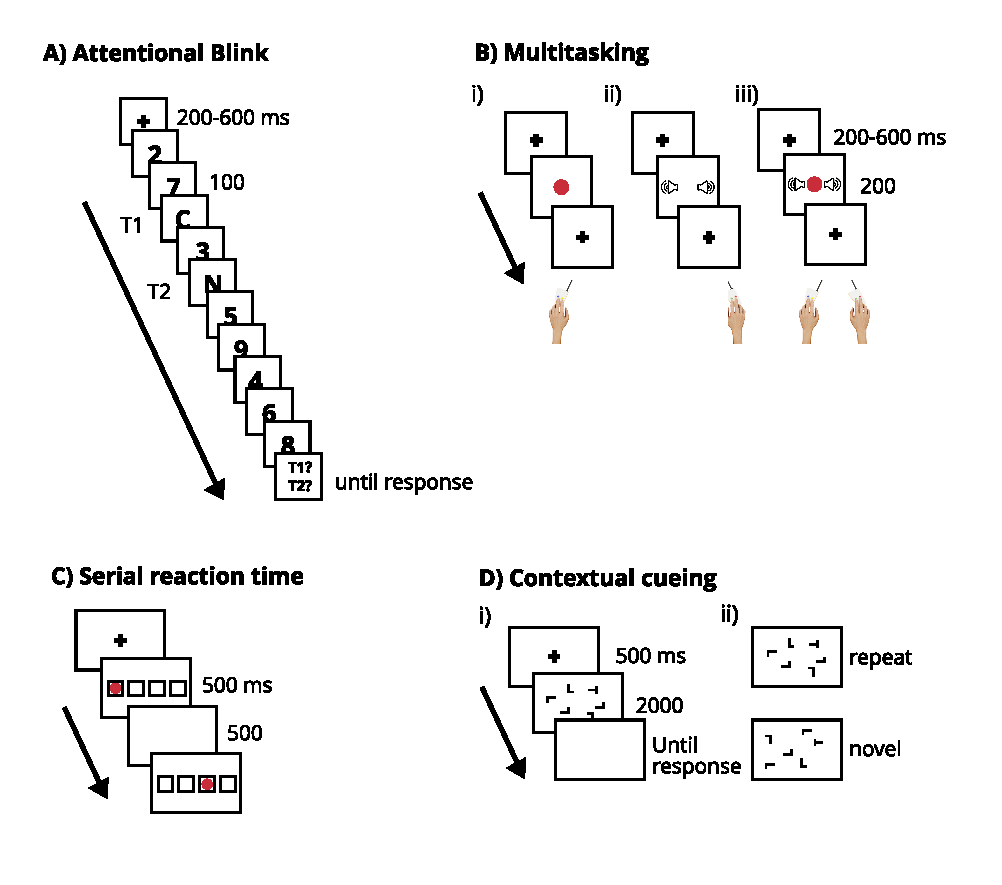
\includegraphics[width=0.7\linewidth]{../images/FigXXXX_alltasks} 

}

\caption{Task battery. A) Attentional Blink Paradigm (AB). Participants report the two letter targets from the rapid serial visual presentation of numbers and letters, B) Multitasking Paradigm (MT). Participants make a discriminate the colour of a disc, a complex tone, or both C) Contextual Cueing Paradigm (CC). i) Participants perform an inefficient visual search task. ii) Unknown to participants, half of the search arrays are repeated throughout the course of the experiment. D) Serial reaction time task (SRT). Participants respond to one of four stimuli, each mapped to a spatially-compatible button press. Unknown to participants, for half of the blocks the stimulus follows a repeating sequence. E) Visual Statistical Learning Paradigm (VSL): i) 12 shapes are grouped into 6 base pairs. ii) Learning: three of the six pairs are presented as an array, this is repeated as participants passively view the displays. iii) Test: participants are presented with a base pair, and a novel pair formed from a recombination of the 12 shapes, and is asked which of the two pairs they have seen previously.}\label{fig:fig:FigureParadigm}
\end{figure}

All the \href{}{data} and
\href{https://github.com/kel-github/Super-Effects}{code} used for the
current analysis are available online. The analysis of the data from
each task followed two steps. First, to ascertain that we observed the
typical findings for each of the paradigms, we applied the conventional
statistical model for that to the full dataset (N=313). The details of
each analysis are presented below. Next, we implemented a simulation
procedure to determine the effect size and p-values that would be
attained over many experiments conducted at multiple levels of sample
size.

\hypertarget{sampling-procedure}{%
\subsubsection{Sampling procedure}\label{sampling-procedure}}

For each task, we sampled across 20 different sample sizes (\(N\)s),
defined on a logarithmic interval between N=13 and N=313. We opted for a
logarithmic interval given the decreasing information gained at higher
\(N\) values. To simulate \(k\) experiments at each of our chosen \(N\),
we developed a sampling procedure that sought to leverage information
from across the whole dataset while also protecting against any
reductions in effect size variablility that may be attributable to
saturation as \(N\) approaches the maximum (\(N_{max}\)=313).
Specifically, it could be that as \(N\) approaches 313, the overlap of
participants between subsamples may be greater than when \(N\) equals a
lower number such as 13. It follows then that any decreasing variability
in effect size estimates at higher \(N\)s could be due to the decrease
in variability of the subsamples, rather than the improved estimate of
the population variance should come with a larger \(N\).

To protect against this possibility we applied the following procedure;
for each level of \(N\) (\(N_{1}, N_{2}, ...N_{20}\)), we first selected
a subsample from the total dataset \emph{without} replacement,
e.g.~\(N\) of 13 unique samples from the total \(N\)=313. We refer to
this from now on as the \emph{parent subsample}. From this parent
subsample, we sampled \(k\) = 1000 times \emph{with} replacement -
e.g.~\(N\)=13 sampled from \(N\)=13. These shall now be referred to as
the \emph{child subsamples}. The relevant analysis was then applied to
each of the child subsamples. Sampling with replacement ensured that the
child subsamples carried the Markov property. Given that this procedure
reduces the heterogeneity of the parent sample (for example, in the case
of \(N\)=13, all the child subsamples are derived from only 13 unique
observations), we then repeated the entire process over \(j\) = 1000
iterations. Therefore the presented data reflects \(j * k\) simulated
experiments for each level of \(N\). We refer to this now as the
two-step sampling procedure: \(j\) = 1000, \(k\) = 1000. It is worth
noting that we compared this procedure to one where we performed the
two-step sampling procedure with \(j\) = 1, and to a one-step sampling
procedure where we sampled \(N\) with replacement from the entire
dataset, i.e.~\(k\)=1000 and \(j\) = 0. Outcomes were comparable between
the sampling procedures, with the two-step procedure (\(j\) = 1000)
offering better resolution of the resulting densities (see Figure
\ref{fig:samples} for a representative example).

\begin{verbatim}
## `summarise()` regrouping output by 'samp', 'mod' (override with `.groups` argument)
\end{verbatim}

\begin{center}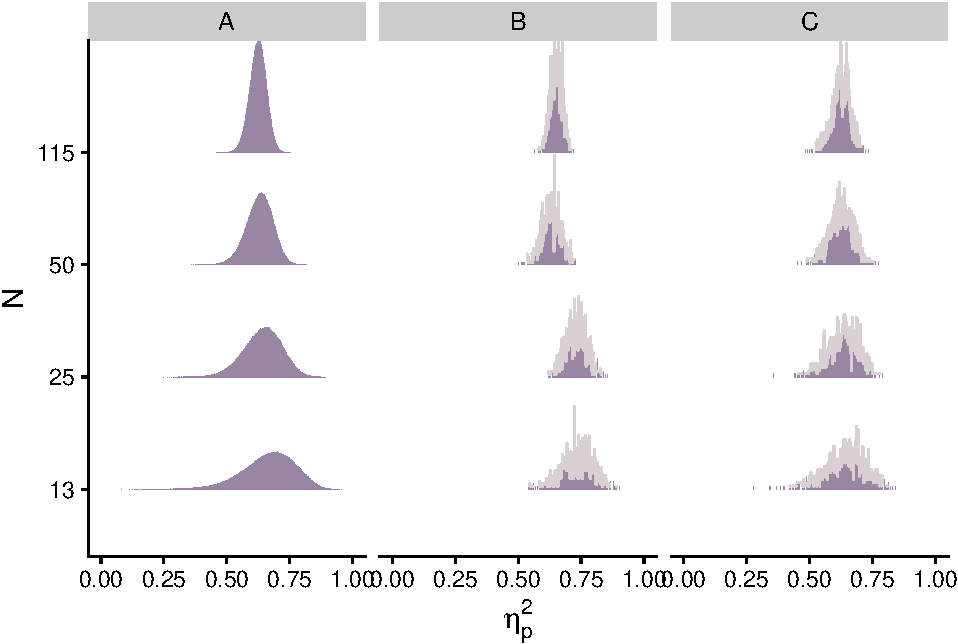
\includegraphics[width=0.7\linewidth]{super-fx_files/figure-latex/supp_sampling-1} \end{center}

\begin{figure}
  \centering
  \caption{Comparison between sampling procedures for the AB task data fit with a repeated measures ANOVA for 4 levels of N; densities of observed effect sizes for the A) two-step sampling procedure $j$=1000, $k$=1000, the B) two-step sampling procedure, $j$=1, $k$=1000, and C) the one-step procedure, $k$ = 1000}
  \label{fig:samples}
\end{figure}

\[
\xi _{ij}(t)=P(x_{t}=i,x_{t+1}=j|y,v,w;\theta)= {\frac {\alpha _{i}(t)a^{w_t}_{ij}\beta _{j}(t+1)b^{v_{t+1}}_{j}(y_{t+1})}{\sum _{i=1}^{N} \sum _{j=1}^{N} \alpha _{i}(t)a^{w_t}_{ij}\beta _{j}(t+1)b^{v_{t+1}}_{j}(y_{t+1})}}
\]

\hypertarget{headings-third-level}{%
\subsubsection{Headings: third level}\label{headings-third-level}}

\lipsum[6]

\paragraph{Paragraph}
\lipsum[7]

\hypertarget{examples-of-citations-figures-tables-references}{%
\section{Examples of citations, figures, tables,
references}\label{examples-of-citations-figures-tables-references}}

\label{sec:others}

\lipsum[8] some text ({\textbf{???}}; {\textbf{???}}) and see
({\textbf{???}}).

The documentation for \verb+natbib+ may be found at

\begin{center}
  \url{http://mirrors.ctan.org/macros/latex/contrib/natbib/natnotes.pdf}
\end{center}

Of note is the command \verb+\citet+, which produces citations
appropriate for use in inline text. For example,

\begin{verbatim}
   \citet{hasselmo} investigated\dots
\end{verbatim}

produces

\begin{quote}
  Hasselmo, et al.\ (1995) investigated\dots
\end{quote}

\begin{center}
  \url{https://www.ctan.org/pkg/booktabs}
\end{center}

\hypertarget{figures}{%
\subsection{Figures}\label{figures}}

\lipsum[10] See Figure \ref{fig:fig1}. Here is how you add footnotes.
{[}\^{}Sample of the first footnote.{]}

\lipsum[11]

\begin{figure}
  \centering
  \fbox{\rule[-.5cm]{4cm}{4cm} \rule[-.5cm]{4cm}{0cm}}
  \caption{Sample figure caption.}
  \label{fig:fig1}
\end{figure}

\begin{center}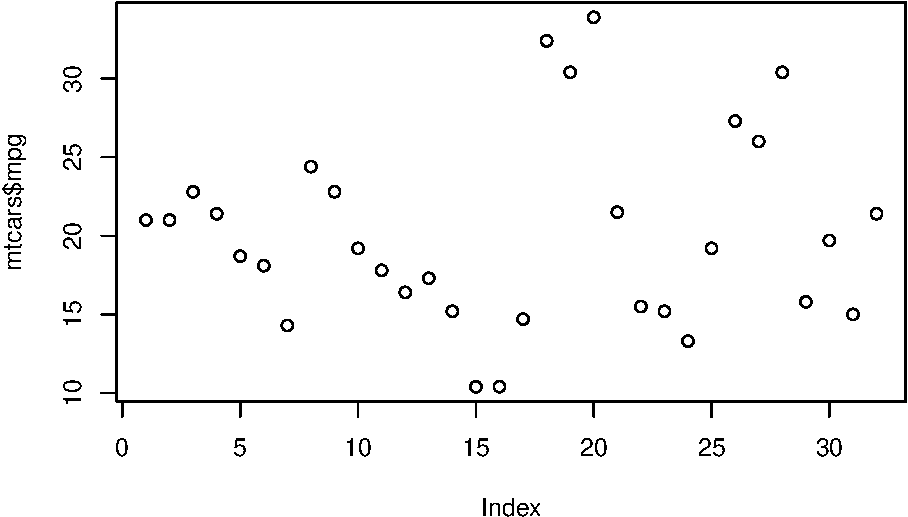
\includegraphics{super-fx_files/figure-latex/unnamed-chunk-1-1} \end{center}

\hypertarget{tables}{%
\subsection{Tables}\label{tables}}

\lipsum[12]

See awesome Table\textasciitilde{}\ref{tab:table}.

\begin{table}
 \caption{Sample table title}
  \centering
  \begin{tabular}{lll}
    \toprule
    \multicolumn{2}{c}{Part}                   \\
    \cmidrule(r){1-2}
    Name     & Description     & Size ($\mu$m) \\
    \midrule
    Dendrite & Input terminal  & $\sim$100     \\
    Axon     & Output terminal & $\sim$10      \\
    Soma     & Cell body       & up to $10^6$  \\
    \bottomrule
  \end{tabular}
  \label{tab:table}
\end{table}

\hypertarget{lists}{%
\subsection{Lists}\label{lists}}

\begin{itemize}
\tightlist
\item
  Lorem ipsum dolor sit amet
\item
  consectetur adipiscing elit.
\item
  Aliquam dignissim blandit est, in dictum tortor gravida eget. In ac
  rutrum magna.
\end{itemize}

\hypertarget{refs}{}
\begin{cslreferences}
\leavevmode\hypertarget{ref-bagiellaMixedeffectsModelsPsychophysiology2000}{}%
Bagiella, Emilia, Richard P. Sloan, and Daniel F. Heitjan. 2000.
``Mixed-Effects Models in Psychophysiology.'' \emph{Psychophysiology} 37
(1): 13--20.
\url{https://doi.org/https://doi.org/10.1111/1469-8986.3710013}.

\leavevmode\hypertarget{ref-brainardPsychophysicsToolbox1997}{}%
Brainard, D. H. 1997. ``The Psychophysics Toolbox.'' \emph{Spatial
Vision} 10 (4): 433--36.

\leavevmode\hypertarget{ref-brysbaertPowerAnalysisEffect2018}{}%
Brysbaert, Marc, and Michaël Stevens. 2018. ``Power Analysis and Effect
Size in Mixed Effects Models: A Tutorial.'' \emph{Journal of Cognition}
1 (1): 9. \url{https://doi.org/10.5334/joc.10}.

\leavevmode\hypertarget{ref-mccullochRepeatedMeasuresANOVA2005}{}%
McCulloch, Charles E. 2005. ``Repeated Measures ANOVA, R.I.P.?''
\emph{CHANCE} 18 (3): 29--33.
\url{https://doi.org/10.1080/09332480.2005.10722732}.

\leavevmode\hypertarget{ref-muthAlternativeModelsSmall2016}{}%
Muth, Chelsea, Karen L. Bales, Katie Hinde, Nicole Maninger, Sally P.
Mendoza, and Emilio Ferrer. 2016. ``Alternative Models for Small Samples
in Psychological Research: Applying Linear Mixed Effects Models and
Generalized Estimating Equations to Repeated Measures Data.''
\emph{Educational and Psychological Measurement} 76 (1): 64--87.
\url{https://doi.org/10.1177/0013164415580432}.

\leavevmode\hypertarget{ref-pelliVideoToolboxSoftwareVisual1997}{}%
Pelli, Denis G. 1997. ``The VideoToolbox Software for Visual
Psychophysics: Transforming Numbers into Movies.'' \emph{Spatial Vision}
10 (4): 437--42. \url{https://doi.org/10.1163/156856897X00366}.
\end{cslreferences}

\bibliographystyle{unsrt}
\bibliography{refs.bib}


\end{document}
